\subsection{Эффективный потенцал}

Квадрат скорости тела на орбите массы $m$ может быть выражен как сумма квадратов \imp{лучевой} и \imp{трансверсальной} скоростей. Запишем закон сохранения энергии в следующей форме:
\begin{equation*}
	\frac{m(v^2_r + v^2_{\perp})}{2} - \frac{GMm}{r} = E_0,
\end{equation*}
где $E_0$~--- полная энергия тела на данной орбите. Вспомним выражение для модуля момента импульса:
\begin{equation}
	L = r p_{\perp} = mr v_{\perp}.
\end{equation}
Выразим $v_{\perp}$ через $L$ и подставим в ЗСЭ.
\begin{equation}
	\frac{m v^2_r}{2} + \frac{L^2}{2mr^2} - \frac{GMm}{r} = E_0.
\end{equation}
Эффективным потенциалом системы $\tilde{U}(r)$ называется выражение
\begin{equation}
	\tilde{U}(r) = \frac{L^2}{2mr^2} - \frac{GMm}{r}.
\end{equation}
Рассмотрим случай $v_r=0$ (перицентр или апоцентр орбиты). В таких точках полная энергия тела в точности равна $\tilde{U}(r)$.

\begin{wrapfigure}[10]{r}{0.47\tw}
    \centering
%    \vspace{-1pc}
    \tikzsetnextfilename{effitient-potential-plot}
    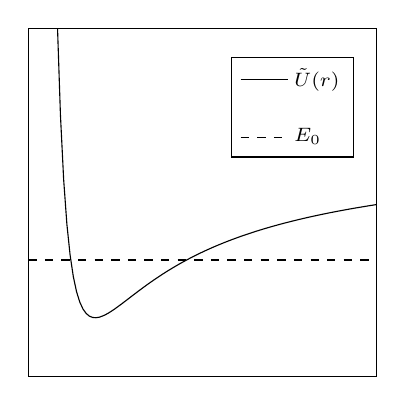
\begin{tikzpicture}
        \begin{axis}[
            width    =    6cm,
            height    =    6cm,
%            xlabel    =    {$r$},
%            xlabel style = {at={(axis description cs:0.5,-0.1)}}
            ymax    =    1,
            ymin    =    -2,
            xmax    =    3,
            xmin    =    0,
            ticks = none,
            legend cell align=left,
            legend style={
                row sep = 0.8pc,
                font=\scriptsize,
                at={(axis cs:1.75, 0.75)}, anchor=north west,
            },
        ]
            \addplot [domain=0.25:3, samples=100, black] {1 / (2 * x^2) - 1.73 / x};
            \addplot [dashed, line width=0.5pt] coordinates { (0,-1) (3,-1) };

            \legend{
                $\tilde{U}(r)$,
                $E_0$
            }
        \end{axis}
    \end{tikzpicture}
    \caption{Эффективный потенциал}
    \label{pic:effitient-potential-plot}
\end{wrapfigure} 

Исходя из \picRef{pic:effitient-potential-plot} при $E_0<0$ существует две различных интересующих нас величины $r$. 
%Так как данные точки соответствуют перицентру и апоцентру орбиты запишем эту пару как $r_{\pi}$ и $r_{\alpha}$ соответственно.
Решим уравнение $\tilde{U}(r) = E_0$, корнями которого являются $r_{\pi}$ и $r_{\alpha}$:
\begin{gather*}
	\frac{L^2}{2mr^2} - \frac{GMm}{r} = E_0 \\
	r^2 + \frac{GMm}{E_0}r - \frac{L^2}{2m E_0} = 0
\end{gather*}
По теореме Виета для корней данного квадратного уравнения можно записать следующие соотношения:
\begin{equation*}
\left\{\begin{aligned}
&r_\pi+r_\alpha=2 a & =-\frac{G M m}{E_0} \\
&r_\pi r_\alpha=b^2 & =-\frac{L^2}{2 m E_0} .
\end{aligned}\right.
\end{equation*}
Решив данную систему уравнений, получим выражения для $E_0$ и $L$:
\begin{gather}
	L = m \sqrt{GMp}, \\
	E_0 = -\frac{GMm}{2a}.
	\label{eq:total-orbit-energy}
\end{gather}







